\documentclass[prd,twocolumn,superscriptaddress,nofootinbib,amsmath,amssymb,floatfix]{revtex4-2}
%DIF LATEXDIFF DIFFERENCE FILE
%DIF DEL toolkit-1p1-v4.tex   Sat Oct 31 08:45:51 2026
%DIF ADD toolkit-1p1-v5.tex   Sat Oct 31 09:01:57 2026
\usepackage{graphicx}
\usepackage{xcolor}
\graphicspath{{../figs/}}
\usepackage{booktabs}
\usepackage{tikz}
\usepackage[colorlinks=true,linkcolor=blue!50!black,citecolor=blue!50!black,urlcolor=blue!50!black]{hyperref}
\newcommand{\pending}[1]{\textcolor{red}{[#1]}}
\definecolor{bandA}{HTML}{008A7C}
\definecolor{bandB}{HTML}{C2610C}

% 1+1 paper, split from counting-full-v2.tex (session 15, 2026-10-29). Companion: embedding-3p1-v1.tex; methodology: methodology-note-v1.tex.
% Rules (Roberto): PRD register; failed attempts only in App. A (deletable); AI use = short disclosure + citation of the methodology note.
% Round 2 (referee agent): reframed as "exact identities and their deviations"; baseline table (r31); Laguerre vs fixed-n related fraction (r32);
% propagator section moved before the embedding test; claims softened; qualifiers restored.
% v2 (session 17, external referee round 1, CQG track; answer in ~/Desktop/papers/1+1 CQG/answers/answer-toolkit-1p1-v2.md): restructured around
% Secs. III-IV; Laguerre target moved to Appendix A (Roberto); Table II with Hu-Meyer-Meyer and the bias-correction ablation (r36); curvature:
% count-defined window, pooled estimator (the v1 offset was a ratio bias), sprinkled pairs, BD / chain-abundance noise (r37), FRW kernel (r38).
% Placeholders (\pending): Zenodo DOI (at submission). r27 filled in v4 (session 19).
% v3 (session 18, external referee round 2, answer in ~/Desktop/papers/1+1 CQG/answers/answer-toolkit-1p1-v3.md): sprinkled-pair shortfall traced to
% nearest-element selection (r40 select); order-only window in a causally convex region (r40 convex); FRW test with the pooled estimator (r40 frw);
% noise in realistic use, P pairs in one diamond vs ordering fraction (r40 noise); kernel = first moment only; tau^4 systematic; refs; version refs removed.
% v4 (session 19, external referee round 3, answer in ~/Desktop/papers/1+1 CQG/answers/answer-toolkit-1p1-v4.md): abstract matched to Sec. IV (in-region
% bias, less precise than the ordering fraction); Mecke condition stated, count-defined example removed; one-region comparison rerun with a position-based
% selection and a flat control at matched element count (r41); FRW shortfall 26-35 %; convexity argument without f, convexity as an assumption;
% data availability worded as a commitment; Discussion: the curvature result is analytic and conceptual (optional locality test not run).
% v5 (session 20, external referee round 4 = accept after 25-29; answer in ~/Desktop/papers/1+1 CQG/answers/answer-toolkit-1p1-v5.md): abstract %DIF > 
% 'coefficients summed over the pairs of many sprinklings'; Fig. 3 cut stated (stricter than the fit window); flat-control lever arm; unrounded %DIF > 
% inserted-pair offsets; N = 800 test: M, threshold, height context, small sample, full-test count 4/20 in Limitations; present tense; Last-Penrose cited. %DIF > 
%DIF PREAMBLE EXTENSION ADDED BY LATEXDIFF
%DIF UNDERLINE PREAMBLE %DIF PREAMBLE
\RequirePackage[normalem]{ulem} %DIF PREAMBLE
\RequirePackage{color}\definecolor{RED}{rgb}{1,0,0}\definecolor{BLUE}{rgb}{0,0,1} %DIF PREAMBLE
\providecommand{\DIFaddtex}[1]{{\protect\color{blue}\uwave{#1}}} %DIF PREAMBLE
\providecommand{\DIFdeltex}[1]{{\protect\color{red}\sout{#1}}} %DIF PREAMBLE
%DIF SAFE PREAMBLE %DIF PREAMBLE
\providecommand{\DIFaddbegin}{} %DIF PREAMBLE
\providecommand{\DIFaddend}{} %DIF PREAMBLE
\providecommand{\DIFdelbegin}{} %DIF PREAMBLE
\providecommand{\DIFdelend}{} %DIF PREAMBLE
\providecommand{\DIFmodbegin}{} %DIF PREAMBLE
\providecommand{\DIFmodend}{} %DIF PREAMBLE
%DIF FLOATSAFE PREAMBLE %DIF PREAMBLE
\providecommand{\DIFaddFL}[1]{\DIFadd{#1}} %DIF PREAMBLE
\providecommand{\DIFdelFL}[1]{\DIFdel{#1}} %DIF PREAMBLE
\providecommand{\DIFaddbeginFL}{} %DIF PREAMBLE
\providecommand{\DIFaddendFL}{} %DIF PREAMBLE
\providecommand{\DIFdelbeginFL}{} %DIF PREAMBLE
\providecommand{\DIFdelendFL}{} %DIF PREAMBLE
%DIF HYPERREF PREAMBLE %DIF PREAMBLE
\providecommand{\DIFadd}[1]{\texorpdfstring{\DIFaddtex{#1}}{#1}} %DIF PREAMBLE
\providecommand{\DIFdel}[1]{\texorpdfstring{\DIFdeltex{#1}}{}} %DIF PREAMBLE
\providecommand{\DIFscaledelfig}{0.5}
%DIF HIGHLIGHTGRAPHICS PREAMBLE %DIF PREAMBLE
\RequirePackage{settobox} %DIF PREAMBLE
\RequirePackage{letltxmacro} %DIF PREAMBLE
\newsavebox{\DIFdelgraphicsbox} %DIF PREAMBLE
\newlength{\DIFdelgraphicswidth} %DIF PREAMBLE
\newlength{\DIFdelgraphicsheight} %DIF PREAMBLE
% store original definition of \includegraphics %DIF PREAMBLE
\LetLtxMacro{\DIFOincludegraphics}{\includegraphics} %DIF PREAMBLE
\providecommand{\DIFaddincludegraphics}[2][]{{\color{blue}\fbox{\DIFOincludegraphics[#1]{#2}}}} %DIF PREAMBLE
\providecommand{\DIFdelincludegraphics}[2][]{% %DIF PREAMBLE
\sbox{\DIFdelgraphicsbox}{\DIFOincludegraphics[#1]{#2}}% %DIF PREAMBLE
\settoboxwidth{\DIFdelgraphicswidth}{\DIFdelgraphicsbox} %DIF PREAMBLE
\settoboxtotalheight{\DIFdelgraphicsheight}{\DIFdelgraphicsbox} %DIF PREAMBLE
\scalebox{\DIFscaledelfig}{% %DIF PREAMBLE
\parbox[b]{\DIFdelgraphicswidth}{\usebox{\DIFdelgraphicsbox}\\[-\baselineskip] \rule{\DIFdelgraphicswidth}{0em}}\llap{\resizebox{\DIFdelgraphicswidth}{\DIFdelgraphicsheight}{% %DIF PREAMBLE
\setlength{\unitlength}{\DIFdelgraphicswidth}% %DIF PREAMBLE
\begin{picture}(1,1)% %DIF PREAMBLE
\thicklines\linethickness{2pt} %DIF PREAMBLE
{\color[rgb]{1,0,0}\put(0,0){\framebox(1,1){}}}% %DIF PREAMBLE
{\color[rgb]{1,0,0}\put(0,0){\line( 1,1){1}}}% %DIF PREAMBLE
{\color[rgb]{1,0,0}\put(0,1){\line(1,-1){1}}}% %DIF PREAMBLE
\end{picture}% %DIF PREAMBLE
}\hspace*{3pt}}} %DIF PREAMBLE
} %DIF PREAMBLE
\LetLtxMacro{\DIFOaddbegin}{\DIFaddbegin} %DIF PREAMBLE
\LetLtxMacro{\DIFOaddend}{\DIFaddend} %DIF PREAMBLE
\LetLtxMacro{\DIFOdelbegin}{\DIFdelbegin} %DIF PREAMBLE
\LetLtxMacro{\DIFOdelend}{\DIFdelend} %DIF PREAMBLE
\DeclareRobustCommand{\DIFaddbegin}{\DIFOaddbegin \let\includegraphics\DIFaddincludegraphics} %DIF PREAMBLE
\DeclareRobustCommand{\DIFaddend}{\DIFOaddend \let\includegraphics\DIFOincludegraphics} %DIF PREAMBLE
\DeclareRobustCommand{\DIFdelbegin}{\DIFOdelbegin \let\includegraphics\DIFdelincludegraphics} %DIF PREAMBLE
\DeclareRobustCommand{\DIFdelend}{\DIFOaddend \let\includegraphics\DIFOincludegraphics} %DIF PREAMBLE
\LetLtxMacro{\DIFOaddbeginFL}{\DIFaddbeginFL} %DIF PREAMBLE
\LetLtxMacro{\DIFOaddendFL}{\DIFaddendFL} %DIF PREAMBLE
\LetLtxMacro{\DIFOdelbeginFL}{\DIFdelbeginFL} %DIF PREAMBLE
\LetLtxMacro{\DIFOdelendFL}{\DIFdelendFL} %DIF PREAMBLE
\DeclareRobustCommand{\DIFaddbeginFL}{\DIFOaddbeginFL \let\includegraphics\DIFaddincludegraphics} %DIF PREAMBLE
\DeclareRobustCommand{\DIFaddendFL}{\DIFOaddendFL \let\includegraphics\DIFOincludegraphics} %DIF PREAMBLE
\DeclareRobustCommand{\DIFdelbeginFL}{\DIFOdelbeginFL \let\includegraphics\DIFdelincludegraphics} %DIF PREAMBLE
\DeclareRobustCommand{\DIFdelendFL}{\DIFOaddendFL \let\includegraphics\DIFOincludegraphics} %DIF PREAMBLE
%DIF AMSMATHULEM PREAMBLE %DIF PREAMBLE
\makeatletter %DIF PREAMBLE
\let\sout@orig\sout %DIF PREAMBLE
\renewcommand{\sout}[1]{\ifmmode\text{\sout@orig{\ensuremath{#1}}}\else\sout@orig{#1}\fi} %DIF PREAMBLE
\makeatother %DIF PREAMBLE
%DIF END PREAMBLE EXTENSION ADDED BY LATEXDIFF

\begin{document}

\title{Spatial distance and curvature from an exact counting identity in two-dimensional causal sets}

\author{Roberto Bada}
\email{roberto@sapereia.com}
\affiliation{SapereIA, Barcelona, Spain}
\affiliation{Institute of Cosmos Sciences, University of Barcelona (ICCUB), Barcelona, Spain}

\date{\today}

\begin{abstract}
In causal set theory, geometry must be recovered from the causal order and from counting. In two dimensions, the causal-overlap regions of Bogu\~n\'a and Krioukov satisfy an exact identity: for two spacelike elements and \emph{any} element $c$ in their common past, $d^2=2V_AV_B/V_C$ in flat spacetime. With a Poisson bias correction it gives a spatial-distance estimator that is unbiased for $d^2$ above two discreteness lengths. On the same pairs it is more accurate than the equal-depth construction of Bogu\~n\'a and Krioukov at all separations, the freedom in the choice of $c$ being what improves on it; between two and ten discreteness lengths it is as accurate as or more accurate than the past--future construction of Hu, Meyer and Meyer, which is more accurate at larger separations. In curved spacetime the identity fails in a way that depends on the depth of $c$. In de Sitter space $d^2_{\rm est}/d^2=\tanh^2(H\tau/2)/[2\ln\cosh(H\tau/2)]=1-R\tau^2/16+O(\tau^4)$, and in any $1+1$ FRW spacetime, to leading order in the depth, the failure measures the scalar curvature one third of the way from the pair to $c$. A fit of this depth drift, \DIFdelbegin \DIFdel{pooled over many pairs , reproduces on average over independent sprinklings}\DIFdelend \DIFaddbegin \DIFadd{with its coefficients summed over the pairs of many independent sprinklings, reproduces }\DIFaddend the same fit on the exact continuum volumes, for pairs inserted by hand (de Sitter, flat and FRW sprinklings) and for all sprinkled pairs of a position-based selection (de Sitter and flat, within $1.7\sigma$); selecting the elements nearest to given points biases it low. On a sprinkling of a causally convex region, such as an interval of the causal set, its window needs no coordinates. For the curvature of a given region, however, it is less precise than the ordering fraction (in de Sitter space its spread between sprinklings is about three times larger) and, within one region, biased low. As a supporting diagnostic we calibrate the Lorentzian-embedding test of Clough and Evans and add the fraction of null-separated pairs, which lets the test reject layered orders on its own. A Laguerre identity for the mean of Johnston's propagator at fixed interval size is given in an appendix.
\end{abstract}

\maketitle

\section{Introduction}\label{sec:intro}
A causal set is a locally finite partially ordered set: every interval $I(x,y)=\{z:x\prec z\prec y\}$ is finite~\cite{BLMS87,Surya19}. Causal set theory proposes that spacetime is such a set, with the continuum emerging at large scales. The number of elements in a region then measures its spacetime volume and the order fixes the light cones; the kinematic programme is to recover all other geometric information from these two ingredients.

Part of this programme is well established. The longest chain between two elements estimates their proper time~\cite{BrightwellGregory91}; interval and chain abundances give the dimension~\cite{Myrheim78,Meyer88} and the curvature~\cite{RSS13,GlaserSurya13}; the Benincasa--Dowker operator gives the scalar curvature and the action~\cite{BD10,DowkerGlaser13}. Spatial distance is harder, because spacelike elements bound no interval. Bogu\~n\'a and Krioukov measured it through the overlap of the pasts of two elements as seen from an element $c$ at equal proper time below both~\cite{BK24}; Brightwell and Gregory and Rideout and Wallden used the smallest interval containing both elements~\cite{BrightwellGregory91,RideoutWallden09}; Hu, Meyer and Meyer gave an exact reconstruction in $1+1$ dimensions from a past and a future element~\cite{HMM25}. Whether a causal set resembles a manifold at all is tested by dimension estimators, interval abundances~\cite{GlaserSurya13} and Lorentzian embeddings~\cite{CloughEvans16,Henson06,Johnston25}. Matter can be introduced through Johnston's sum over chains~\cite{Johnston08,Johnston09}, whose average over sprinklings reproduces the Klein--Gordon propagator.

Two-dimensional causal sets are a natural laboratory: every $1+1$ metric is conformally flat, intervals are rectangles in light-cone coordinates, and a sprinkled diamond is a uniformly random two-dimensional order, whose combinatorics is known~\cite{BHS08,Surya12}; the $e^{-\beta S}$ model of two-dimensional orders also has a well-studied phase structure~\cite{BHS08,Surya12,GOS18}. This paper is built on one exact identity that follows from these facts, and on the use of its violation as a measure of curvature. The \emph{rectangle identity} expresses the spatial distance of two elements through the overlap volumes seen from any element of their common past (Sec.~\ref{sec:dist}). It removes the equal-depth requirement of Ref.~\cite{BK24} and yields a distance estimator, which we compare with the equal-depth, past--future and Hu--Meyer--Meyer constructions on the same pairs. In curved spacetime the identity fails as a function of the depth of $c$; we derive this depth drift in closed form in de Sitter space and to leading order in any $1+1$ FRW spacetime, and turn it into a curvature estimator (Sec.~\ref{sec:curv}). Spatial distance in causal sets has also been approached through thickened antichains and induced distances on spatial hypersurfaces~\cite{MRS06,MRS07,ESV19}, and curvature through interval and chain abundances in small causal diamonds~\cite{RSS13,KhetrapalSurya13} and the Benincasa--Dowker operator~\cite{BD10}; we compare with the last two at equal density.

As a supporting diagnostic we calibrate the Lorentzian-embedding test of Clough and Evans and add a statistic that lets it reject layered orders on its own (Sec.~\ref{sec:embed}), and apply it to sequential growth and to configurations of the $e^{-\beta S}$ model (Sec.~\ref{sec:phases}). Section~\ref{sec:disc} discusses novelty and limitations. Appendix~\ref{app:prop} gives a combinatorial identity for Johnston's propagator at fixed interval size, and Appendix~\ref{app:dropped} summarizes other approaches we tested. Spatial distances in $3+1$ dimensions, where the rectangle identity has no analogue, are treated in a companion paper~\cite{Embedding}.

\section{Setting}\label{sec:setting}
Test causal sets are generated by sprinkling: a Poisson process of density $\rho$ in a region of a given spacetime, with the order induced by the light cones. The coordinates are then discarded and used only for comparison. We write $\ell=\rho^{-1/2}$ for the discreteness length: a region of volume $\ell^2$ contains one element on average.

We use light-cone coordinates $u=t-x$, $v=t+x$, in which $dt\,dx=du\,dv/2$ and $x\prec y$ if and only if $u_x<u_y$ and $v_x<v_y$. The interval between $x\prec y$ is the rectangle $[u_x,u_y]\times[v_x,v_y]$, with volume $V=\Delta u\,\Delta v/2=\tau^2/2$. A sprinkled causal diamond is therefore a uniformly random two-dimensional order, the intersection of two random linear orders~\cite{BHS08,Surya12}. For two spacelike elements, $d^2=\Delta x^2-\Delta t^2=-\Delta u\,\Delta v$.

The proper time from the longest chain has mean $\simeq2\sqrt n$ in an interval of $n$ elements, with Tracy--Widom fluctuations of order $n^{1/6}$~\cite{BDJ99}; wherever a volume is available we use the count instead, $\tau^2=2n/\rho$. Pairs of elements in one sprinkling share elements and their errors are correlated; quoted uncertainties are therefore computed from the spread between independent sprinklings.

\section{The rectangle identity and a distance estimator}\label{sec:dist}
Let $a,b$ be spacelike and $c$ an element in their common past. Following Ref.~\cite{BK24}, we split the two intervals into
\begin{equation}
\begin{gathered}
A=I(c,a)\setminus I(c,b),\qquad B=I(c,b)\setminus I(c,a),\\
C=I(c,a)\cap I(c,b).
\end{gathered}
\end{equation}
Bogu\~n\'a and Krioukov choose $c$ at equal proper time below $a$ and $b$ and derive $d$ from the overlap fraction. In $1+1$ dimensions the choice of $c$ is immaterial, because of the following identity (Fig.~\ref{fig:tiles}).

\begin{figure}[t]
\centering
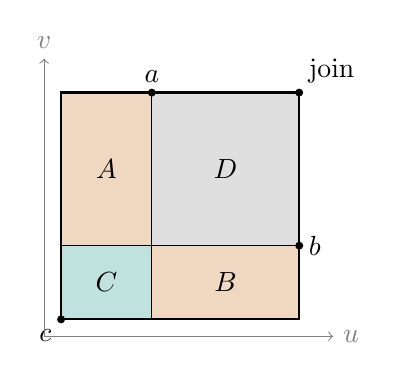
\begin{tikzpicture}[scale=0.72]
  \fill[bandA!25] (0,0) rectangle (1.6,1.3);
  \fill[bandB!25] (0,1.3) rectangle (1.6,4);
  \fill[bandB!25] (1.6,0) rectangle (4.2,1.3);
  \fill[gray!25] (1.6,1.3) rectangle (4.2,4);
  \draw[thick] (0,0) rectangle (4.2,4);
  \draw (1.6,0) -- (1.6,4); \draw (0,1.3) -- (4.2,1.3);
  \node at (0.8,0.65) {$C$}; \node at (0.8,2.65) {$A$}; \node at (2.9,0.65) {$B$}; \node at (2.9,2.65) {$D$};
  \fill (0,0) circle (2pt) node[below left] {$c$};
  \fill (1.6,4) circle (2pt) node[above] {$a$};
  \fill (4.2,1.3) circle (2pt) node[right] {$b$};
  \fill (4.2,4) circle (2pt) node[above right] {join};
  \draw[->,gray] (-0.3,-0.3) -- (4.8,-0.3) node[right] {$u$};
  \draw[->,gray] (-0.3,-0.3) -- (-0.3,4.6) node[above] {$v$};
\end{tikzpicture}
\caption{The rectangle identity in light-cone coordinates (rotated by $45^\circ$ with respect to the usual picture). The rectangle from $c$ to the join of $a$ and $b$ splits into the overlap $C$, the strips $A$ and $B$ seen by only one of $a,b$, and the tile $D$ with $a$ and $b$ at opposite corners. Opposite tiles have equal products, $V_CV_D=V_AV_B$, and $V_D=d^2/2$.}
\label{fig:tiles}
\end{figure}

\emph{Derivation.} Place $c$ at the origin and take $u_a<u_b$, $v_a>v_b$ ($a$ and $b$ spacelike). Then $I(c,a)=[0,u_a]\times[0,v_a]$ and $I(c,b)=[0,u_b]\times[0,v_b]$. The rectangle from $c$ to the join $(u_b,v_a)$ splits into four tiles,
\begin{equation}
\begin{aligned}
C&=[0,u_a]\times[0,v_b], & A&=[0,u_a]\times[v_b,v_a],\\
B&=[u_a,u_b]\times[0,v_b], & D&=[u_a,u_b]\times[v_b,v_a].
\end{aligned}
\end{equation}
With $\Delta u=u_b-u_a$ and $\Delta v=v_a-v_b$, the volumes are $V_C=u_av_b/2$, $V_A=u_a\Delta v/2$, $V_B=\Delta u\,v_b/2$, $V_D=\Delta u\,\Delta v/2$, so that $V_CV_D=V_AV_B$. The tile $D$ has $a$ and $b$ at opposite corners, so $V_D=d^2/2$. Hence, for every $c$ in the common past,
\begin{equation}
d^2=\frac{2V_AV_B}{V_C}.
\label{eq:rect}
\end{equation}
The tile $D$ is the interval between the meet and the join of $a$ and $b$, i.e., the region whose volume defines the $1+1$ spatial distance of Brightwell and Gregory and of Rideout and Wallden~\cite{BrightwellGregory91,RideoutWallden09}. The identity shows that this volume can be read from the past alone, through a single element $c$. The equal-time choice of Ref.~\cite{BK24} is $V_A=V_B$, in which case their $1+1$ formula reduces to Eq.~\eqref{eq:rect}; for general $c$ the search for equal-time elements, which requires the density and the dimension, is unnecessary. The identity relies on the overlap of two $1+1$ intervals being again an interval; in higher dimensions it is not, and Eq.~\eqref{eq:rect} has no direct analogue.

\emph{Estimator.} On a causal set, $V_X$ is replaced by $N_X/\rho$, the number of elements in the region. The three regions are disjoint, so $N_A$, $N_B$, $N_C$ are independent Poisson variables with means $\lambda_X=\rho V_X$. The product $N_AN_B$ is unbiased for $\lambda_A\lambda_B$, but $1/N_C$ is biased and undefined at $N_C=0$. Since $E[1/(N+1)]=(1-e^{-\lambda})/\lambda$ for a Poisson variable,
\begin{equation}
\widehat{d^2}=\frac{2N_AN_B}{\rho\,(N_C+1)}
\label{eq:est}
\end{equation}
is unbiased for $d^2$ up to a factor $1-e^{-\lambda_C}$. The relative variance is approximately $1/\lambda_A+1/\lambda_B+1/\lambda_C$, so the deepest available $c$ is optimal; we take the element with the largest $N_C$. The strips $A$ and $B$ are long and thin and contain many elements even when $d\sim\ell$, which is why the estimator works down to the discreteness scale; by contrast, a direct count of the tile $D$ has relative variance $1/\lambda_D=2\ell^2/d^2$, which is $\tfrac12$ at $d=2\ell$.

\emph{Tests.} Two pair selections are used, and the difference matters for the size of the errors: Table~\ref{tab:dist} and Fig.~\ref{fig:distance} use random spacelike pairs among \emph{late} elements of flat sprinklings of a unit diamond, which have large common pasts; Table~\ref{tab:base} uses pairs in the \emph{middle} of the diamond, which have both a common past and a common future but smaller ones. In both, $c$ is the deepest element for each pair. The median error falls approximately as $N^{-1/2}$ at large $d$, and remains at $15$--$25\%$ below $2\ell$, the discreteness scale itself, where $\widehat{d^2}$ is also biased high [by $(37\pm7)\%$ at $N=4000$ on the pairs of Table~\ref{tab:base}]. Table~\ref{tab:base} compares the estimator with the existing constructions on the same pairs: the equal-depth filter of Bogu\~n\'a and Krioukov [their Eq.~(34)]; the smallest interval $I(c,f)$ with $c\prec a,b\prec f$ (Brightwell--Gregory, Rideout--Wallden), $d^2=2(N_{\min}-2)/\rho$; and the construction of Hu, Meyer and Meyer~\cite{HMM25}, who showed that for $p\prec a,b\prec q$ with all four proper times equal to $s$, $d^2=\tau_{pq}^2-4s^2$. They gave it as an exact statement about Minkowski space; on the causal set we read every $\tau^2$ from a count ($\tau^2=2N/\rho$), take $p$ from the common past and $q$ from the common future, keep the pairs $(p,q)$ whose four counts agree within Poisson noise ($\chi^2<3$), and among them use the one with the smallest counts, which has the smallest variance (choosing instead the best-matched or averaging over all matched pairs is less accurate). Two ablations separate the ingredients of our estimator: the same deepest $c$ without the Poisson correction, $2N_AN_B/\rho N_C$, and the equal-depth elements $c$ of Ref.~\cite{BK24} with the corrected formula, Eq.~\eqref{eq:est}.

Above $2\ell$ the rectangle estimator is unbiased for $d^2$ within the uncertainties. Between $2\ell$ and $10\ell$ its median error is the smallest; the Hu--Meyer--Meyer estimate is close in error but biased high by about $20\%$, because $\tau_{pq}^2-4s^2$ is a small difference of two noisy terms. Above $10\ell$ the Hu--Meyer--Meyer estimate is unbiased and the most accurate, with half the error of ours or less: there the tile between $a$ and $b$ is large, and a direct count of it, corrected exactly by the four equal intervals, beats reading the same volume from the strips. For $d$ itself the rectangle estimator reads $1$--$3.5\%$ low, as expected from the square root of an unbiased estimate of $d^2$. The plain past--future count is biased high, because the smallest interval between elements cannot coincide with the tile $D$. The ablations locate the gain over the equal-depth estimator. With the deepest $c$, $N_C$ is large and the Poisson correction makes no difference. With the equal-depth elements, where $N_C$ is small, the correction removes the bias of the equal-depth estimator ($+10\%\to+1\%$ and $+6\%\to+2\%$ between $2\ell$ and $10\ell$), but not its larger error ($0.129$ and $0.104$, against $0.095$ and $0.059$ with the deepest $c$). The bias of Ref.~\cite{BK24} on the causal set thus comes from the uncorrected ratio of small counts, and the accuracy gain from the freedom to use the deepest $c$, which the identity provides. The equal-depth filter also returns no estimate for $10$--$30\%$ of the pairs. Below $2\ell$ every estimator is poor, and the two past--future constructions fail entirely (median errors above $50\%$). For the baseline tests we add a bottom element that precedes all others; the deepest $c$ is then always that element, selected without reference to its own count, so the selection introduces no bias (in Table~\ref{tab:dist}, without such an element, it is one of the lowest elements); the freedom in the choice of $c$ is exercised by the curvature tests of Sec.~\ref{sec:curv}.

\begin{table}[t]
\caption{Median relative error of Eq.~\eqref{eq:est} with the deepest $c$; flat $1+1$ sprinklings, 300 pairs among late elements in each of 4 sprinklings per $N$. (Table~\ref{tab:base} uses pairs in the middle of the diamond, with smaller common pasts, and therefore larger errors.)}
\label{tab:dist}
\begin{ruledtabular}
\begin{tabular}{rccc}
$N$ & $d<2\ell$ & $2\ell$--$10\ell$ & $>10\ell$\\
\hline
1000 & 23\% & 6.5\% & 5.2\%\\
2000 & 15\% & 5.0\% & 3.4\%\\
4000 & 19\% & 5.1\% & 2.5\%\\
\end{tabular}
\end{ruledtabular}
\end{table}

\begin{table}[t]
\caption{Rectangle estimator, Eq.~\eqref{eq:est}, against the equal-depth filter of Ref.~\cite{BK24}, the past--future construction of Hu, Meyer and Meyer~\cite{HMM25} read from counts (see text), and the smallest past--future interval~\cite{BrightwellGregory91,RideoutWallden09}, on the same spacelike pairs in the middle of flat diamonds (12 sprinklings $\times$ 100 pairs per $N$). Two ablations: the deepest $c$ without the Poisson correction, and the equal-depth elements $c$ with it. Bias: mean relative error of $d^2$, in percent, with the standard error from the spread between sprinklings in parentheses. Error: median absolute relative error of $d$. The equal-depth rows have no estimate for $10$--$30\%$ of the pairs.}
\label{tab:base}
\begin{ruledtabular}
\begin{tabular}{llcccc}
 & & \multicolumn{2}{c}{$2\ell$--$10\ell$} & \multicolumn{2}{c}{$>10\ell$}\\
$N$ & method & bias & error & bias & error\\
\hline
1000 & rectangle, Eq.~\eqref{eq:est} & $+1(5)$ & 0.095 & $-4(4)$ & 0.082\\
 & \quad no correction & $+3(5)$ & 0.097 & $+1(4)$ & 0.080\\
 & equal depth~\cite{BK24} & $+10(4)$ & 0.131 & $+13(3)$ & 0.126\\
 & \quad with correction & $+1(3)$ & 0.129 & $-2(3)$ & 0.127\\
 & Hu--Meyer--Meyer & $+23(3)$ & 0.098 & $+4(2)$ & 0.028\\
 & past--future & $+86(3)$ & 0.272 & $+25(3)$ & 0.095\\
4000 & rectangle, Eq.~\eqref{eq:est} & $0(2)$ & 0.059 & $-2(1)$ & 0.039\\
 & \quad no correction & $0(2)$ & 0.059 & $0(2)$ & 0.037\\
 & equal depth~\cite{BK24} & $+6(2)$ & 0.106 & $+2(1)$ & 0.075\\
 & \quad with correction & $+2(2)$ & 0.104 & $-5(1)$ & 0.073\\
 & Hu--Meyer--Meyer & $+22(4)$ & 0.099 & $0(1)$ & 0.015\\
 & past--future & $+79(5)$ & 0.282 & $+14(1)$ & 0.049\\
\end{tabular}
\end{ruledtabular}
\end{table}

\begin{figure}[t]
\centering
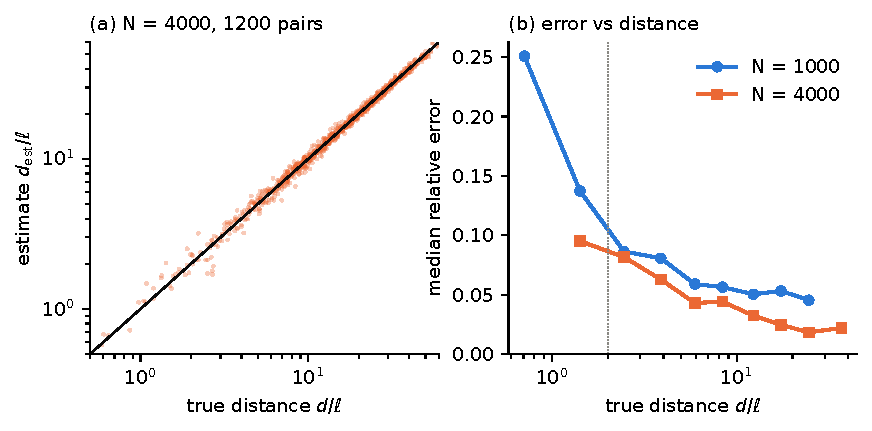
\includegraphics[width=\columnwidth]{fig_distance}
\caption{Eq.~\eqref{eq:est} with the deepest $c$ on flat $1+1$ sprinklings, from the causal order only. (a) Estimate against true distance, $N=4000$. (b) Median relative error per distance bin; the dotted line marks $2\ell$.}
\label{fig:distance}
\end{figure}

\section{Curvature from depth drift}\label{sec:curv}
In flat spacetime every $c$ in the common past gives the same estimate. In curved spacetime Eq.~\eqref{eq:rect} no longer holds exactly, and the estimate depends on the depth of $c$. This dependence measures curvature.

\emph{de Sitter volumes.} Two-dimensional de Sitter space in conformal coordinates,
\begin{equation}
ds^2=\frac{-d\eta^2+dx^2}{(H\eta)^2},\qquad\eta<0,
\end{equation}
has the light cones of flat space. The tiles $A,B,C,D$ are the same rectangles in $(u,v)=(\eta-x,\eta+x)$, but volumes carry the conformal weight,
\begin{equation}
dV=\frac{d\eta\,dx}{(H\eta)^2}=\frac{2\,du\,dv}{H^2(u+v)^2}.
\end{equation}
Integrating over $[u_1,u_2]\times[v_1,v_2]$, the inner integral gives $1/(u+v_1)-1/(u+v_2)$ and the outer one a logarithm,
\begin{equation}
V_\square=\frac{2}{H^2}\ln\frac{\eta_L\,\eta_R}{\eta_{\rm bot}\,\eta_{\rm top}},
\label{eq:dsvol}
\end{equation}
with $\eta=(u+v)/2$ evaluated at the left, right, bottom and top corners (all $\eta<0$, so the argument is positive).

\emph{Closed form.} Place $a,b$ on one slice at $(\eta_0,\mp h)$ and $c$ directly below their midpoint at $(\eta_0-T,0)$, and set $H=1$. By symmetry $V_A=V_B$. Writing $\bar\eta=|\eta_0|$ and $q=\bar\eta+T/2$ (so that $|\eta|$ at the corners of $A$ is $q\mp h/2$, $\bar\eta+h$ and $\bar\eta$), Eq.~\eqref{eq:dsvol} gives, to first order in $h$,
\begin{equation}
V_A=2\ln\frac{(q-\tfrac h2)(\bar\eta+h)}{(q+\tfrac h2)\,\bar\eta}\simeq2h\Big(\frac{1}{\bar\eta}-\frac{1}{q}\Big)=\frac{hT}{\bar\eta\,q},
\end{equation}
and at $h=0$
\begin{equation}
V_C=2\ln\frac{q^2}{(\bar\eta+T)\,\bar\eta}=-2\ln(1-x),\qquad x=\frac{T^2}{4q^2}.
\end{equation}
The true distance is $d\simeq2h/\bar\eta$, so
\begin{equation}
\frac{d^2_{\rm est}}{d^2}=\frac{2V_A^2/V_C}{4h^2/\bar\eta^2}=\frac{x}{-\ln(1-x)}.
\end{equation}
The proper time from $c$ to the midpoint of $a,b$ is $\tau=\ln[(\bar\eta+T)/\bar\eta]$, so that $T/\bar\eta=e^{\tau}-1$ and $x=[(e^\tau-1)/(e^\tau+1)]^2=\tanh^2(\tau/2)$. Restoring $H$,
\begin{equation}
\begin{aligned}
\frac{d^2_{\rm est}}{d^2}&=\frac{\tanh^2(H\tau/2)}{2\ln\cosh(H\tau/2)}=1-\frac{(H\tau)^2}{8}+O(\tau^4)\\
&=1-\frac{R\,\tau^2}{16}+\dots,\qquad R=2H^2,
\end{aligned}
\label{eq:drift}
\end{equation}
exact as $d\to0$ at any depth, for $c$ directly below the midpoint of $a$ and $b$. The denominator is $H^2/2$ times the de Sitter volume of an interval of height $\tau$, $V=(4/H^2)\ln\cosh(H\tau/2)$, and the result is independent of $\eta_0$, as required by the de Sitter symmetry. We verified Eq.~\eqref{eq:drift} against the exact volumes of Eq.~\eqref{eq:dsvol} to $10^{-5}$ for $H\tau=0.1$--$3$. A sideways offset of $c$ changes it little, and a finite $d$ adds an approximately depth-independent shift. We call $1-d^2_{\rm est}/d^2$ the depth drift.

\emph{Other spacetimes.} Every $1+1$ metric is conformally flat, so the leading term should hold locally in any $1+1$ spacetime. We checked this in FRW spacetimes $ds^2=a(\eta)^2(-d\eta^2+dx^2)$ with $a=\eta^p$, where $R=2(\ln a)''/a^2=-2p\,\eta^{-2-2p}$ varies in time and the rectangle volumes have closed forms. For $p=1$, $-2$ and $\tfrac12$ (negative, positive and negative curvature), $16(1-d^2_{\rm est}/d^2)/\tau^2$ tends to $R$ at the location of $a,b$ as $\tau\to0$ (to $1\%$ at $\tau=0.01$), with the correct sign: for $R<0$ the ratio exceeds $1$. At finite depth it measures a curvature between the values at $a,b$ and at $c$, with more weight near the top. The weighting follows from the next order. Write $a=e^{\sigma(\eta)}$, place $a,b$ at $(\eta_0,\mp h)$ and $c$ a coordinate time $T$ straight below. As $h\to0$ the strips have $V_A=V_B=h\int_0^Te^{2\sigma(\eta_0-s/2)}ds$, the overlap is $V_C=\tfrac12\int_0^T\!\!\int_0^Te^{2\sigma(\eta_0-(s+r)/2)}ds\,dr$, and $d=2he^{\sigma(\eta_0)}$. Expanding $\sigma$ in a Taylor series at $\eta_0$, integrating term by term, and trading $T$ for the proper time $\tau=\int_0^Te^{\sigma(\eta_0-s)}ds$ gives
\begin{equation}
1-\frac{d^2_{\rm est}}{d^2}=\frac{\tau^2}{16}\Big[R-\frac{\tau}{3}\,\frac{dR}{d\tau}+O(\tau^2)\Big],
\label{eq:kernel}
\end{equation}
with $R=2\sigma''e^{-2\sigma}$ and its derivative along the worldline (toward the future) evaluated at $a,b$. To this order the drift measures $R$ one third of the way from $a,b$ down to $c$. Only this first moment of the depth weighting is fixed by Eq.~\eqref{eq:kernel}; a triangular weight $2(\tau-s)/\tau^2$ on the depths $s\in[0,\tau]$ is one illustration with this mean depth, not a kernel determined by the expansion, whose next order involves $R^2$ and $d^2R/d\tau^2$ and is not of the form of a weighted average of $R$. The exact power-law volumes confirm Eq.~\eqref{eq:kernel}: for $p=1$ at $\eta_0=1.5$, $16(1-d^2_{\rm est}/d^2)/\tau^2=-0.3982$, $-0.4073$, $-0.4200$ at $\tau=0.02$, $0.05$, $0.1$, against $-0.3997$, $-0.4068$, $-0.4185$ from its two terms ($R=-0.395$ at $a,b$); the other two values of $p$ agree equally well.

\emph{Test on sprinklings.} We sprinkle de Sitter space ($H=1$, $\rho=10^4$) and, as a control, flat space in the same coordinates, insert $a,b$ by hand $\approx14\ell$ apart, and evaluate Eq.~\eqref{eq:est} for every sprinkled $c$ in their common past \DIFdelbegin \DIFdel{whose rectangle lies inside }\DIFdelend \DIFaddbegin \DIFadd{such that the smallest rectangle containing $I(c,a)$ and $I(c,b)$ lies in }\DIFaddend the region. \DIFaddbegin \DIFadd{This cut is stricter than the window of the fit below, which requires only the two intervals to lie in the region. }\DIFaddend Figure~\ref{fig:drift} shows the mean ratio per depth bin over 400 sprinklings against the continuum value computed for the same elements $c$, which includes the effects of finite $d$ and of sideways offsets and therefore lies slightly below Eq.~\eqref{eq:drift}. The flat control remains at $1$ and de Sitter follows the continuum. Neighboring depth bins share elements: computed from the spread over the 400 sprinklings, the correlation of adjacent bins is $0.80$, $0.81$, $0.90$, $0.94$, $0.96$ in de Sitter space (from the shallowest pair to the deepest) and $0.80$--$0.97$ in flat space, and bins two apart are still correlated at $0.5$--$0.9$. A run of deviations in adjacent bins therefore counts as a single fluctuation, and the points of Fig.~\ref{fig:drift} must not be combined as independent. In the shallowest bin the tile $C$ contains few elements, the factor $1-e^{-\lambda_C}$ of Eq.~\eqref{eq:est} is not negligible, and the estimator reads low in both geometries.

\begin{figure}[t]
\centering
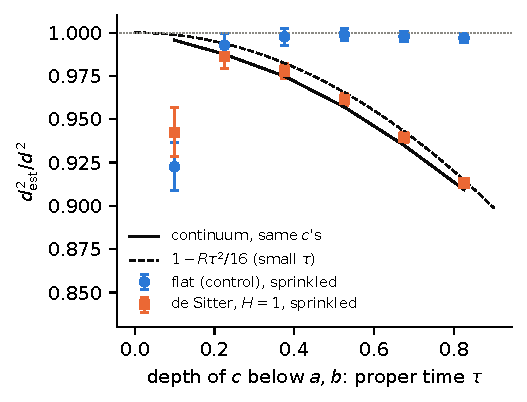
\includegraphics[width=0.85\columnwidth]{fig_drift}
\caption{Depth drift of the rectangle estimate: mean over 400 sprinklings ($\rho=10^4$, $H=1$) per bin of the proper time $\tau$ from $c$ to $a,b$, with errors from the spread between sprinklings. The bins are strongly correlated (adjacent bins $0.8$--$0.97$; see text), so the error bars are not independent. Solid: continuum ratio from the exact volumes, averaged over the same elements $c$ (finite $d$ and offsets included). Dashed: small-$\tau$ term of Eq.~\eqref{eq:drift}.}
\label{fig:drift}
\end{figure}

\emph{A curvature estimator.} For one pair $a,b$ we fit $\widehat{d^2}=\alpha+\beta\tau^2$ over the elements $c$ of their common past, with $\tau^2=(N_{I(c,a)}+N_{I(c,b)})/\rho$ from counts, and read $R=-16\beta/\alpha$. Two choices need care.

\emph{Window from the order.} The fit uses every $c$ with $N_C\geq20$, which keeps the factor $1-e^{-\lambda_C}$ of Eq.~\eqref{eq:est} negligible, down to the deepest $c$ whose intervals $I(c,a)$ and $I(c,b)$ lie in the sprinkled region. Neither limit refers to $H$. The estimator counts only $A$, $B$ and $C$, which lie in $I(c,a)\cup I(c,b)$; the tile $D$ is never counted. In a causally convex region that contains $c$, $a$ and $b$, these intervals lie in the region. On a sprinkling of a causally convex region, for example an interval of the causal set, every $c$ in the common past can therefore be used, so the window needs no coordinates; otherwise the boundary must first be inferred, which in $1+1$ dimensions is possible from the order~\cite{Cunningham18}. Convexity is an assumption about the sprinkled region: the order decides it only when the causal set is itself defined from the order, as an interval is. Our main tests use a coordinate box, where we decide the condition from the coordinates. We therefore repeated them in a causally convex region, the past of the point $(-0.95,0)$ cut at $\eta=-3$ (convex, although the cut is not defined by the order), with every $c$ of the common past used (1000 sprinklings each). The results agree with Table~\ref{tab:rest}: in de Sitter space the pooled estimate is $2.10\pm0.09$ and $2.03\pm0.06$ with inserted pairs and $2.10\pm0.08$ and $2.04\pm0.06$ with all pairs in the windows, at $\rho=4000$ and $10^4$, against continuum values $2.03$ and $2.04$ (the deeper region changes the target, see below); in flat space $0.01\pm0.02$ and $0.00\pm0.02$ at $\rho=4000$, and $0.00\pm0.01$ and $-0.01\pm0.01$ at $\rho=10^4$. Because this window reaches $H\tau\approx1$, the $\tau^4$ term of Eq.~\eqref{eq:drift} contributes, and the same fit applied to the exact continuum volumes of the same elements gives $R_{\rm fit}^{\rm cont}=2.07$--$2.08$ in the de Sitter box (and $2.03$--$2.04$ in the convex region) instead of $2$. This, not $2$, is the value the estimator reproduces; since it is not known in practice, the difference is a systematic of the method, of $+2$ to $+4\%$ here, which depends on the size of the region. Varying the lower cut ($N_C\geq5$, $20$, $50$) and the upper cut ($\tau^2$ up to $50\%$, $75\%$ or $100\%$ of its largest value) changes the pooled de Sitter result only between $1.91$ and $2.01$ at $\rho=10^4$ (flat: $-0.01$ to $0.00$), within $0.06$--$0.28$ of the continuum value of each rule; the largest offset belongs to the shortest window, which is also the noisiest.

\emph{Pooling.} A single pair gives a noisy estimate (standard deviation $3.5$ at $\rho=4000$ and $2.4$ at $\rho=10^4$ in de Sitter space), and the mean of single-pair values is biased low: the intercept and slope of one least-squares fit have anticorrelated errors, so $E[-16\beta/\alpha]$ is smaller than $-16E[\beta]/E[\alpha]$. Summing the fit coefficients over the pairs before forming the ratio, $R_{\rm est}=-16\sum\beta/\sum\alpha$, removes this ratio bias to first order. Table~\ref{tab:rest} shows the pooled estimator over 1000 sprinklings, with errors from a bootstrap over sprinklings. With inserted pairs it agrees with the continuum value of the same fit, in flat space within the errors and in de Sitter space within \DIFaddbegin \DIFadd{$0.9\sigma$ and }\DIFaddend $1.1\sigma$ \DIFdelbegin \DIFdel{at both densities}\DIFdelend \DIFaddbegin \DIFadd{(offsets $-0.095\pm0.111$ and $-0.081\pm0.072$ before rounding)}\DIFaddend .

\emph{Sprinkled pairs.} How $a$ and $b$ are chosen among the sprinkled elements matters. Taking the elements nearest to two target points selects elements with an empty neighbourhood (the nearest point lies on the boundary of an empty disc), and part of that disc lies at the shallow ends of the strips $A$ and $B$. The counts confirm it: averaged over the elements $c$ of the window, $N_A-\rho V_A$ is lower by $0.2$--$0.4$ elements than for inserted pairs, at every depth. Since $\lambda_A$ grows with the depth of $c$, a fixed deficit lowers $\widehat{d^2}$ most for shallow $c$, which tilts the fitted slope upward and gives $R$ low, in flat space as well; the effect shrinks with density. With this selection the estimator reads low in de Sitter space by $0.37\pm0.11$ at $\rho=4000$ and $0.24\pm0.07$ at $\rho=10^4$ (Table~\ref{tab:rest}). The unbiased use of sprinkled pairs follows from the Mecke formula\DIFaddbegin \DIFadd{~\mbox{%DIFAUXCMD
\cite{LastPenrose17}}\hskip0pt%DIFAUXCMD
}\DIFaddend : a sum over all pairs of points of a Poisson process, with a weight that depends only on the positions of the pair and not on the rest of the configuration, equals the average over pairs placed by hand at the same positions. The condition is therefore a sum over all pairs of a selection that does not depend on the counts used by the estimator, optionally thinned at random with a fixed probability; the ratio is formed from the pooled sums. We therefore take every spacelike pair with $a$ in a square window of half-width $0.025$ around one target point and $b$ in the window around the other ($\approx2.5\ell$ at $\rho=10^4$), keep each pair with a fixed probability chosen so that about $20$ pairs per sprinkling remain, and pool them all. This removes most of the shortfall: the pooled estimate is $1.91\pm0.10$ and $2.02\pm0.06$ in de Sitter space against continuum values $2.08$ ($1.7\sigma$ and $1.1\sigma$ below, against $0.9\sigma$ and $1.1\sigma$ for inserted pairs), and $0.00\pm0.02$ and $-0.01\pm0.01$ in flat space (Table~\ref{tab:rest}); in the causally convex region it is $2.10\pm0.08$ and $2.04\pm0.06$ against $2.03$ and $2.04$. Drawing a single pair uniformly from the two windows lies in between ($1.80\pm0.11$ and $1.90\pm0.07$): choosing one element out of the $N_W$ in a window weights each configuration by $1/N_W$, which removes about one element from the window. In practice, therefore, the estimator is to be pooled over all pairs of a position-based selection, not over a single representative chosen per region. A selection by count-defined separation does not satisfy the condition, because it depends on the same counts as the estimator, and we have not tested it.

\emph{FRW spacetime.} We repeated the test in the $p=1$ FRW spacetime ($\rho=10^4$, 1000 sprinklings), with $a,b$ inserted $14\ell$ apart at $\eta_0=1.5$, the pooled estimator and the window of the previous paragraphs, in a causally convex region (the past of an element at $\eta=1.55$) cut at three depths. With windows reaching $\tau=0.52$, $0.70$ and $0.84$, over which $R$ ranges from $-0.40$ at $a,b$ to $-1.37$, $-2.79$ and $-6.32$, the pooled estimate is $-1.03\pm0.37$, $-0.88\pm0.18$ and $-0.93\pm0.11$, against $-0.70$, $-0.79$ and $-0.90$ for the same fit on the exact volumes of the same elements: the estimator reproduces its continuum target within $1\sigma$. That target is not the leading-order prediction of Eq.~\eqref{eq:kernel}, which gives $-0.52$, $-0.55$ and $-0.59$ when fitted in the same way. For the middle window the difference splits about evenly between the higher orders in $\tau$ (the exact volumes with $c$ straight below and $d\to0$ give $-0.67$) and the finite separation of $a$ and $b$ (with $d=14\ell$ the same curve gives $-0.80$). Over a realistic window Eq.~\eqref{eq:kernel} therefore gives the direction of the effect, a curvature measured below the pair, but falls short of its size by $26$--$35\%$ in the three windows; the size is set by the exact continuum fit, which the counts reproduce.

\emph{Comparison with other estimators.} The Benincasa--Dowker operator~\cite{BD10}, in its nonlocal two-dimensional form with smearing parameter $\epsilon$, applied to a constant field at the midpoint of the pair, gives $R=-2B_\epsilon[1]$. On the de Sitter and flat sprinklings above, its single-point standard deviation at $\rho=4000$ is $\approx1.2\times10^3$, $160$ and $23$--$30$ for $\epsilon=0.1$, $0.03$ and $0.01$, and larger at $\rho=10^4$ ($72$--$82$ at $\epsilon=0.01$), as expected at fixed $\epsilon$. Stronger smearing lowers the spread ($2.7$--$4.5$ at $\epsilon=0.003$), but then the operator needs the past light cone far beyond our sprinkled region, and the truncation dominates its mean ($+0.7$ in flat space, $+4.7$ in de Sitter space); a fair comparison at small $\epsilon$ needs a much larger region, which we have not run. Its purpose is the action rather than a pointwise curvature estimate.

The relevant competitor is the ordering fraction of a causal diamond, the leading chain-abundance route~\cite{RSS13}, compared here as the methods would be used: one sprinkled region, one estimate. The region is a causal diamond (an interval of the causal set) in de Sitter space, $u,v\in[-3,-0.95]$ ($H=1$; $2.5\times10^3$ elements at $\rho=4000$, $6.3\times10^3$ at $\rho=10^4$), sprinkled 400 times. In each sprinkling we take every spacelike pair with $a$ near the top of the diamond ($\eta_a\in[-1.25,-1.05]$, $|x_a|\leq0.1$) and $b$ at $x_b-x_a\in[0.1,0.2]$, $|\eta_b-\eta_a|\leq0.05$ ($9\ell$--$17\ell$ apart at $\rho=10^4$), keep each with a fixed probability, the same in every sprinkling, chosen so that $P$ pairs remain on average (a position-based selection in the sense above), and pool the depth drift over them. We compare with $R=2(f-\tfrac12)/(f_{\rm cont}-\tfrac12)$ from the ordering fraction $f$ of the whole diamond, calibrated on the exact continuum diamond ($f_{\rm cont}=0.5173$). The errors are the spread between sprinklings. As mean and standard deviation, the ordering fraction gives $2.05\pm0.80$ at $\rho=4000$ and $1.99\pm0.46$ at $\rho=10^4$; the pooled drift gives $1.67\pm2.32$ and $1.95\pm1.34$ for $P=100$, against continuum values $2.10$ of the same fit: its spread is about three times larger. Pooling more pairs barely helps (standard deviation $2.78$, $2.50$, $2.32$, $2.27$ for $P=10$, $30$, $100$, $300$ at $\rho=4000$), because pairs in one region share most of their common pasts. For the same reason the ratio bias is not averaged away within one region: the estimate reads low by $0.43\pm0.12$ and $0.15\pm0.07$. It is the ratio that is biased, not the sums: forming the ratio from $\sum\beta$ and $\sum\alpha$ pooled over all 400 sprinklings gives $1.96\pm0.12$ and $2.04\pm0.07$. Drawing the pairs one at a time instead ($a$ uniformly among the elements near the top, then $b$ uniformly among those at the required offset) gives the same within the errors in de Sitter space ($1.63$ and $1.92$). In a flat diamond of the same coordinate size, at a lower density so that it holds the same number of elements as the de Sitter diamond ($2.5\times10^3$ and $6.3\times10^3$), the ordering fraction gives $0.01\pm0.80$ and $0.03\pm0.50$, and the pooled drift $-0.16\pm0.89$ and $-0.05\pm0.54$ (low by $0.16\pm0.04$ and $0.05\pm0.03$). \DIFaddbegin \DIFadd{The flat control is matched in element count, not in proper depth: in the same coordinates the deepest $c$ lies about $1.85$ below the pairs in flat space, against $\ln(3/1.15)\approx0.96$ in de Sitter space, so the range of $\tau^2$ over which the drift is fitted is about four times longer. That alone makes the flat drift less noisy, so the difference between the two geometries in the factors below largely reflects this lever arm, not curvature. }\DIFaddend As a curvature estimator for a given region, the ordering fraction is therefore more precise, by a factor of about three in de Sitter space and slightly in flat space, and less biased. What the depth drift adds is geometric: the curvature appears as the failure of an exact flat-space identity, it is measured along a specific pair and depth rather than over a whole diamond, and Eq.~\eqref{eq:kernel} says where. Other counting routes use Ollivier--Ricci curvature~\cite{BBR26}, which we have not compared.

\begin{table}[t]
\caption{Pooled curvature estimator $R_{\rm est}=-16\sum\beta/\sum\alpha$ over 1000 sprinklings ($H=1$; window as in Sec.~\ref{sec:curv}: $N_C\geq20$, down to the deepest $c$ with $I(c,a)$ and $I(c,b)$ in the box). Pairs: inserted by hand at two target points; (nearest) the sprinkled elements nearest to them; (windows) all spacelike pairs of sprinkled elements in windows around them, about 20 per sprinkling (see text). Errors: bootstrap over sprinklings. $R_{\rm fit}^{\rm cont}$: the same fit on the exact continuum volumes of the same elements (de Sitter). Last column: standard deviation of single-pair values (de Sitter).}
\label{tab:rest}
\begin{ruledtabular}
\begin{tabular}{rlcccc}
$\rho$ & pairs & flat & de Sitter & $R_{\rm fit}^{\rm cont}$ & single pair\\
\hline
4000 & inserted & $-0.03\pm0.03$ & $1.97\pm0.11$ & $2.07$ & $3.5$\\
 & nearest & $-0.07\pm0.03$ & $1.70\pm0.11$ & $2.07$ & $3.6$\\
 & windows & $0.00\pm0.02$ & $1.91\pm0.10$ & $2.08$ & $3.5$\\
$10^4$ & inserted & $-0.01\pm0.02$ & $1.99\pm0.07$ & $2.08$ & $2.4$\\
 & nearest & $-0.04\pm0.02$ & $1.84\pm0.07$ & $2.08$ & $2.4$\\
 & windows & $-0.01\pm0.01$ & $2.02\pm0.06$ & $2.08$ & $2.4$\\
\end{tabular}
\end{ruledtabular}
\end{table}

\section{A supporting diagnostic: the embedding test and its blind spot}\label{sec:embed}
\emph{Embedding.} Given the squared intervals $s_{ij}$ between $M$ sampled elements, classical multidimensional scaling (MDS) with a Lorentzian Gram matrix reconstructs coordinates. Clough and Evans applied it to causal sets and proposed its eigenvalue spectrum as a test of dimension and manifoldlikeness~\cite{CloughEvans16,Clough17}. With $s_{ij}=(x_i-x_j)^{\top}\eta\,(x_i-x_j)$, double centering, $G=-\tfrac12JSJ$ with $J=I-\mathbf1\mathbf1^{\top}/M$, gives $G=X\eta X^{\top}$ for the centered coordinates $X$. A $1+1$ Lorentzian set shows one large negative eigenvalue (time), one large positive eigenvalue (space), and the others near zero; the two eigenvectors give coordinates up to a Lorentz transformation.

We supply MDS with counts only: $s=-2N(I)/\rho$ for related pairs and Eq.~\eqref{eq:est} with the deepest $c$ for spacelike pairs. On $M=150$ elements of a flat sprinkling with $N=2000$, positions are recovered to $0.43\pm0.07\,\ell$ across a region $\approx38\ell$ wide, and the best affine map from the reconstructed to the true coordinates, $x_{\rm true}\approx Ax_{\rm rec}+b$, is a Lorentz transformation to within $3$--$10\%$, in the sense that the largest entry of $A^{\top}\eta A-\eta$ is $0.03$--$0.10$ in absolute value. The two large eigenvalues are $\approx\mp2.2$ and all others are below $0.1$, in the coordinate units of the sprinkled region (a unit square in $u,v$).

\emph{Statistics and calibration.} As test statistics we use intrinsic numbers only: $r_+$, the ratio of the second to the first positive eigenvalue; the share of the spectrum in one time and one space direction, $(|\lambda_-|+\lambda_+)/\sum_i|\lambda_i|$; and the \emph{stress}, the rms misfit of the squared intervals by the best $1+1$ Minkowski embedding relative to their rms. The sample consists of the $M=40$ elements with the largest pasts, after removing elements with no common past with the rest. Figure~\ref{fig:detector}(a) shows the calibration on flat universes (random two-dimensional orders): stress and $r_+$ settle only for $N\gtrsim100$ (stress $0.16$, $0.10$, $0.08$ at $N=100$, $200$, $400$), so the test is used only above this size. Curvature raises the stress: for de Sitter diamonds with fixed $N=400$ it stays in the flat band up to $H\tau\approx1$ and reaches $0.25$ at $H\tau=4$ [Fig.~\ref{fig:detector}(c)]. The stress thus tests whether the order is a \emph{flat} sheet, while Sec.~\ref{sec:curv} measures its curvature.

\emph{Blind spot.} Applied to Monte Carlo samples of the $e^{-\beta S}$ model at $N=400$ (Sec.~\ref{sec:phases}), this test passes every continuum-like state \DIFaddbegin \DIFadd{at that size (not at $N=800$; Sec.~\ref{sec:phases}) }\DIFaddend and fails orders with 4 and 7 layers, but it does not reliably flag orders with about 10 layers: at $M=40$ one of seven lies in the flat band and two more just above it, and at $M=80$ two others have stress $0.03$, lower than flat orders. Two effects are responsible. The sample contains only the top one or two layers. And in a layered order most sampled pairs have zero squared interval: linked pairs have $N(I)=0$, and spacelike pairs often have an empty strip, $N_A=0$ or $N_B=0$. MDS fits an all-zero matrix perfectly; a bilayer produces exactly that.

\emph{Null-pair fraction.} We add the fraction $z$ of sampled pairs with zero squared interval, taken as the larger of its values on the top sample and on a sample spread evenly in height (longest chain below the element) over the upper $70\%$ of the order. On sprinklings $z$ decreases with $N$ (median $0.18$, $0.12$, $0.09$ at $N=100$, $200$, $400$) and does not respond to curvature: de Sitter diamonds at $H\tau=4$ give $0.08$--$0.11$. Layered orders give $0.4$--$1$ [Fig.~\ref{fig:detector}(b)]. We flag an order as layered when $z$ exceeds $1.5$ times the flat median at the same $N$. Orders with only 2--3 layers cannot be processed (too few elements share a common past), and the rule counts them as flagged.

\emph{What $z$ adds.} Layered orders are also detected by simpler statistics: the height (number of layers), the ordering fraction and the Myrheim--Meyer dimension~\cite{Myrheim78,Meyer88}, interval abundances~\cite{GlaserSurya13}, and graph observables~\cite{EMLW26}; in the $e^{-\beta S}$ literature the phases are characterized by the action, the ordering fraction, the height and interval abundances~\cite{Surya12,GOS18,GlaserSurya16,Glaser18,Glaser23}. On our states the fixed-size ordering fraction separates the same groups as $z$ (Appendix~\ref{app:prop}). The null-pair fraction does not detect anything these miss. Its role is to make the embedding test usable on its own: without it the test passes some 10-layer orders, so a user who relied on the embedding spectrum alone would accept them. With $z$ the test needs no second statistic, and it uses only quantities the embedding already computes.

\begin{figure*}[t]
\centering
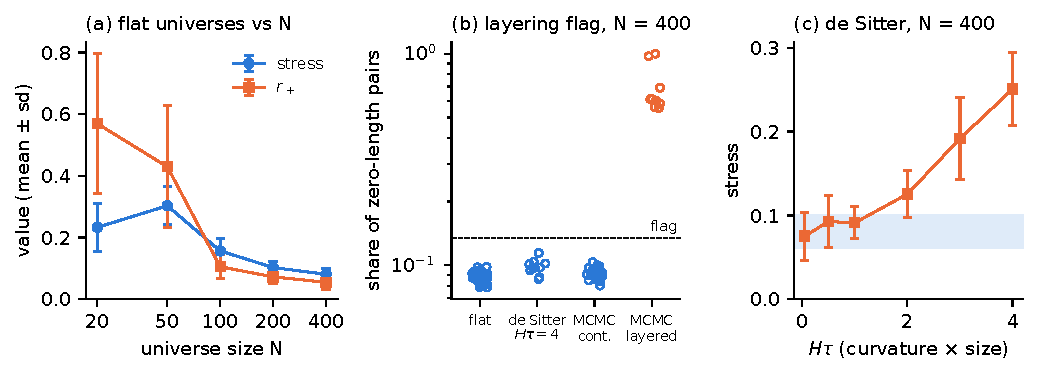
\includegraphics[width=0.9\textwidth]{fig_detector}
\caption{Calibration of the embedding test. (a) Flat universes (random two-dimensional orders, 10 per size, $M=40$): stress and $r_+$ against the number of elements $N$. (b) Null-pair fraction $z$ at $N=400$ ($M=80$) for flat orders, de Sitter diamonds at $H\tau=4$, and final states of $e^{-\beta S}$ Monte Carlo chains (continuum-like, 30--39 layers; layered, 4--11 layers). Dashed: the flag threshold, $1.5$ times the flat median. The 13 states with 2--3 layers are not shown. (c) Stress of de Sitter diamonds at fixed $N=400$ (8 per height) against $H\tau$; shaded: the flat band ($\pm1$ standard deviation).}
\label{fig:detector}
\end{figure*}

\section{Applications}\label{sec:phases}
\emph{Sequential growth.} In transitive percolation, the simplest classical sequential growth model~\cite{RideoutSorkin00}, elements are born one at a time and each newborn element chooses each existing element as an ancestor with probability $p$, and the order is the transitive closure. As a sanity check of the diagnostics we grew universes of $N=100$ and $200$ elements with $p=0.05$, and with the non-covariant variant $p_n=3/n$. Neither produces a $1+1$ spacetime: the ordering-fraction dimension drifts with scale, and the embedding test fails on every statistic (share of the spectrum in one time and one space direction $\approx0.33$ against $0.65$ for flat orders at $N=100$; stress $0.64$--$0.78$ against $0.10$--$0.12$ at $N=200$). Their null-pair fraction is not what flags them; grown universes with $N=1500$ also fail the propagator target (Appendix~\ref{app:prop}). Covariant approaches to cosmology in growth models are discussed in Refs.~\cite{MORS01,AhmedRideout10}.

\emph{The two phases of the $e^{-\beta S}$ model.} Weighting two-dimensional orders by $e^{-\beta S}$, with $S$ the Benincasa--Dowker action, gives a first-order transition between a continuum-like and a layered phase~\cite{BHS08,Surya12,GOS18}. We sampled it with Metropolis swap moves at nonlocality parameter $\epsilon=0.21$ (an $O(N^2)$ update, since a swap changes two rows and columns of the causal matrix). Table~\ref{tab:phases} shows the diagnostics at $N=200$. The states at $\beta\geq0.6$ are metastable intermediates; the ground state at large $\beta$ is a bilayer~\cite{CunninghamSurya19}.

\begin{table}[t]
\caption{Embedding diagnostics on $e^{-\beta S}$ states at $N=200$ ($\epsilon=0.21$). $f$: ordering fraction; $L$: number of layers. The last column gives the range of the null-pair fraction $z$ on fresh chains, for $\beta\le0.3$ (second row) and $\beta\ge0.6$ with 8--13 layers (third row).}
\label{tab:phases}
\begin{ruledtabular}
\begin{tabular}{lccccc}
$N=200$ & $f$ & $L$ & $r_+$ & stress & $z$\\
\hline
random orders & 0.50 & 24 & 0.07 & 0.10 & 0.10--0.15\\
$\beta=0.05$ & 0.51 & 24 & 0.10 & 0.11 & 0.12--0.13\\
$\beta=0.6$ & 0.59 & 9 & 0.39 & 0.28 & 0.39--0.48\\
\end{tabular}
\end{ruledtabular}
\end{table}

The states below are test configurations, representative of the two phases, not equilibrium samples (see the end of this section). We applied the flag to 44 final states of $N=400$ chains run from random and from layered initial orders at $0.01\leq\beta\leq0.7$. All 22 continuum-like states (30--39 layers) pass; all 9 states with 4--11 layers are flagged ($z=0.55$--$1.0$ against a threshold of $0.13$); the 13 states with 2--3 layers cannot be processed and are counted as flagged. The fixed-$n$ ordering fraction (Appendix~\ref{app:prop}) separates the same groups; the propagator statistic misses one 4-layer state. Because the flag was designed after these states had been seen, we tested it on held-out samples. On fresh $N=200$ chains, 12 of 12 continuum-like states pass and 18 of 18 layered states ($\beta=0.6$--$1.5$) are flagged. At $N=800$, with \DIFaddbegin \DIFadd{$M=80$ (as for $z$ at $N=400$) and }\DIFaddend the threshold fixed in advance from flat orders ($z>0.120$\DIFaddbegin \DIFadd{, $1.5$ times the median $z=0.080$ of 50 flat orders}\DIFaddend ; none of 50 fresh flat orders and 20 de Sitter diamonds is flagged), we ran 28 chains ($\beta\in\{0.01,0.05,0.1,0.2,0.3,0.45,0.7\}$, 4 seeds each, random initial orders, 2000 sweeps), with the classes also fixed in advance (at least 20 layers: continuum-like; 4--19 layers: layered). \DIFdelbegin \DIFdel{All }\DIFdelend \DIFaddbegin \DIFadd{On this small held-out sample (}\DIFaddend 8 layered \DIFdelbegin \DIFdel{states }\DIFdelend \DIFaddbegin \DIFadd{and 20 continuum-like states), all 8 layered states }\DIFaddend (14--19 layers) are flagged ($z=0.38$--$0.57$)\DIFdelbegin \DIFdel{, including one whose stress (}\DIFdelend \DIFaddbegin \DIFadd{; only one of them, with stress }\DIFaddend $0.072$\DIFdelbegin \DIFdel{) }\DIFdelend \DIFaddbegin \DIFadd{, }\DIFaddend lies in the flat band, \DIFdelbegin \DIFdel{which the }\DIFdelend \DIFaddbegin \DIFadd{the blind spot that $z$ is meant to close, and the }\DIFaddend embedding spectrum alone would have passed \DIFaddbegin \DIFadd{it}\DIFaddend . Of the 20 continuum-like states (27--56 layers), 19 are not flagged ($z\leq0.107$). The exception has 27 layers at $\beta=0.3$ and is flagged with $z=0.123$, just above the threshold; its acceptance rate ($5\%$, against $53$--$54\%$ for the other three chains at $\beta=0.3$, which reached 43--50 layers) suggests that it is partly layered, but by the classes fixed in advance it is a false positive. \DIFaddbegin \DIFadd{For context only: random two-dimensional orders of $800$ elements have $52$ layers on average (standard deviation $2.5$), so this state has about half the flat height, whereas the continuum-like states at $N=400$ had $30$--$39$ layers against a flat mean of $36$. }\DIFaddend Three of the 19 unflagged states have a stress slightly above the flat band at $N=800$ ($0.086$--$0.110$, against flat mean plus two standard deviations, $0.081$), \DIFaddbegin \DIFadd{as does the flagged one ($0.134$), }\DIFaddend so at this size the stress alone would also reject some continuum-like states. \DIFdelbegin \DIFdel{These }\DIFdelend \DIFaddbegin \DIFadd{The $N=400$ }\DIFaddend states are test inputs, not equilibrium samples: chains started from layered orders accept $\leq0.1\%$ of the moves. They bracket the transition only loosely: chains from layered starts become continuum-like at $\beta\leq0.05$, and chains from random starts become layered at $\beta\geq0.45$. The bracket $0.05<\beta_c(400)<0.45$ is compatible with the finite-size scaling $\beta_c\approx1.66/(\epsilon^2N)=0.094$ of Ref.~\cite{GOS18}; it is too loose to test it.

\section{Discussion}\label{sec:disc}
\emph{What is new.} The overlap regions are those of Ref.~\cite{BK24}, the embedding test is that of Ref.~\cite{CloughEvans16}, the null-pair fraction is related to Ref.~\cite{GlaserSurya13}, and the Laguerre identity is classical combinatorics. To our knowledge the following are new: the rectangle identity for general $c$, Eq.~\eqref{eq:rect}, with the bias-corrected estimator and its comparison with existing constructions, including a counting version of the Hu--Meyer--Meyer construction; the depth drift, its closed form in de Sitter space, Eq.~\eqref{eq:drift}, and its leading form in FRW spacetimes, Eq.~\eqref{eq:kernel}, with the curvature estimator built on it; the application of the Laguerre identity to Johnston's propagator, Eq.~\eqref{eq:lag}; and the calibration of the embedding test against size, curvature and layering. Our literature search (October 2026) covered the citing papers of Refs.~\cite{BK24,CloughEvans16,Johnston08,Johnston09}; the rectangle identity is elementary enough that it may appear in passing in work we did not reach.

\emph{What the curvature result is.} Since the ordering fraction of a region is the more precise estimate of its curvature, the curvature result of this paper is analytic and conceptual: an exact flat-space identity whose depth-dependent failure has a closed form, Eq.~\eqref{eq:drift}, and a leading-order meaning, Eq.~\eqref{eq:kernel}. Whether the locality of the depth drift, a curvature along one pair and one depth, makes it the better estimator where curvature varies across a region is untested. A methodological point is of more general use: estimators evaluated on sprinkled elements chosen as the nearest to given points, or one per window, inherit a Palm-type selection bias, because the choice depends on the neighbourhood that the estimator counts; summing over all elements or pairs of a position-based selection, as the Mecke formula requires, removes it.

\emph{Limitations.} The exact results are specific to $1+1$ dimensions; the rectangle identity has no direct analogue in higher dimensions, where the overlap of two intervals is not an interval. The distance estimator is the most accurate only below about $10\ell$; at larger separations the counting version of the Hu--Meyer--Meyer construction is better. The curvature estimator must be pooled over all pairs of a position-based selection \DIFdelbegin \DIFdel{: single }\DIFdelend \DIFaddbegin \DIFadd{and over many independent regions; within one region the ratio stays biased (below). Single }\DIFaddend pairs are dominated by noise and their ratio is biased, and selecting the elements nearest to given points, or one element per window, biases it low. Its target is the same fit on the continuum volumes, not $R$ itself. Because the window reaches $H\tau\approx1$, the $\tau^4$ term of Eq.~\eqref{eq:drift} makes this target $2.07$--$2.08$ instead of $2$ in our de Sitter box and $2.03$--$2.04$ in the convex region: a systematic of $+2$ to $+4\%$ of the method, which depends on the size of the region and is not known in practice; capping the window lowers it at the cost of noise (Sec.~\ref{sec:curv}). In FRW spacetime the leading-order prediction of Eq.~\eqref{eq:kernel} falls short of this target by $26$--$35\%$ over realistic windows. Within one region the pairs share elements, so pooling more than a few tens of them gains little and the estimate retains a low ratio bias of $0.05$--$0.43$ at the densities used; for the curvature of a given region the ordering fraction is more precise, by a factor of about three in de Sitter space, and less biased. The estimator was tested on de Sitter space and one FRW spacetime. The embedding thresholds are empirical and must be recalibrated at each $N$; on \DIFaddbegin \DIFadd{a small }\DIFaddend held-out \DIFdelbegin \DIFdel{states }\DIFdelend \DIFaddbegin \DIFadd{sample }\DIFaddend at $N=800$ \DIFaddbegin \DIFadd{(8 layered and 20 continuum-like states) }\DIFaddend the layered flag caught every layered state but also one of \DIFaddbegin \DIFadd{the }\DIFaddend 20 continuum-like states, just above its threshold; the \DIFaddbegin \DIFadd{stress put that state ($0.134$) and 3 of the 19 unflagged ones above the flat band, so at this size the full embedding test (spectrum, stress and $z$) rejects 4 of the 20 continuum-like states; the }\DIFaddend $e^{-\beta S}$ states used are test inputs, not equilibrium samples. The Laguerre target is exact only for two-dimensional orders, and as a manifoldlikeness diagnostic it is not stronger than the ordering fraction.

\emph{Outlook.} Since the Hu--Meyer--Meyer construction is the more accurate one at large separations, a depth drift built on it may be less noisy there; a combined distance estimator would switch between the two near $10\ell$. A fixed-$n$ propagator target in $3+1$ dimensions would not be exact: Johnston's $3+1$ particle hops along links only~\cite{Johnston08}, so a path requires every skipped sub-interval to be empty, and $E[K\,|\,n]$ becomes a sum of $(k-1)$-point integrals with factors $(1-W/V)^{n-k+1}$. Its first term can be evaluated at large $n$: the expected number of two-hop link paths tends to $3\pi$, which is what Johnston's amplitudes require to reproduce the short-distance limit $m^2/8\pi$ of the continuum mass term~\cite{Johnston08}, so this is a consistency check rather than a new result; a Monte Carlo evaluation approaches it as $3\pi(1-1.6/\sqrt n)$ at fixed $n$. A $3+1$ target would therefore be a computed table rather than a formula.

\section*{Data availability}
The code that produces every number and figure in this paper, and the research notebook in which the work was carried out, \DIFdelbegin \DIFdel{will be made }\DIFdelend \DIFaddbegin \DIFadd{are }\DIFaddend openly available at \url{https://github.com/presindev/causet-counting}\DIFdelbegin \DIFdel{when this paper is submitted}\DIFdelend , and the version used for this paper \DIFdelbegin \DIFdel{archived with a persistent identifier }\DIFdelend \DIFaddbegin \DIFadd{is archived at doi:}\DIFaddend \pending{Zenodo DOI}. Figures are produced by \texttt{sims/fig\_part1.py}; the baseline comparison by \texttt{sims/r31\_rect\_baseline.py} and, with the Hu--Meyer--Meyer construction and the ablations, \texttt{sims/r36\_rect\_ablation\_hmm.py}; the curvature estimator (window, pooled form, sprinkled pairs, Benincasa--Dowker and chain-abundance comparison, bin correlations) by \texttt{sims/r37\_curvature\_referee.py}; the sprinkled-pair selections, the causally convex region, the FRW test with the pooled estimator and the first comparison with the ordering fraction in one region by \texttt{sims/r40\_curvature\_round2.py}; the one-region comparison with a position-based selection and the flat control at matched element count by \texttt{sims/r41\_curvature\_round3.py}; Eq.~\eqref{eq:kernel} by \texttt{sims/r38\_drift\_kernel.py}; the null-pair fraction by \texttt{sims/r8\_detector\_spread.py}; the curvature fit and the FRW check by \texttt{sims/r9\_drift\_fit\_frw.py}; the $e^{-\beta S}$ states by \texttt{sims/n400\_crystal.py}; the propagator statistics by \texttt{sims/b\_johnston\_n400.py} and \texttt{sims/r32\_laguerre\_vs\_fraction.py}; the $N=800$ test by \texttt{sims/r27\_n800\_detector.py}\DIFaddbegin \DIFadd{, and the heights of random orders quoted with it by }\texttt{\DIFadd{sims/r42\_flat\_height.py}}\DIFaddend .

\begin{acknowledgments}
This work was funded by SapereIA. Simulations were run on the Nyx cluster of the Institute of Cosmos Sciences of the University of Barcelona (ICCUB). An AI system (Claude Opus~5.5, Anthropic) was used for literature search, derivations, code and drafting, under the author's direction and checks; the procedure is described in Ref.~\cite{MethodNote}. The author takes full responsibility for the content.
\end{acknowledgments}

\appendix
\section{A density-free target for Johnston's propagator}\label{app:prop}
This appendix records a combinatorial identity for Johnston's propagator. As a diagnostic of manifoldlikeness it is not stronger than the ordering fraction (end of this appendix); its use is as an exact, density-free check of implementations of the chain sum.

\emph{The propagator.} In Johnston's model a particle hops along the order with amplitude $a$ per hop and $b$ per intermediate stop~\cite{Johnston08}. With $C$ the causal matrix ($C_{xy}=1$ if $x\prec y$) and $\Phi=aC$,
\begin{equation}
K=\Phi+b\,\Phi^2+b^2\Phi^3+\dots=\Phi\,(I-b\Phi)^{-1},
\end{equation}
with $a=\tfrac12$ and $b=-m^2/\rho$ in $1+1$ dimensions. $K(x,y)$ is a weighted count of chains, $K(x,y)=\tfrac12\sum_k c_k(x,y)\,(-\mu/2)^k$, where $c_k$ is the number of $k$-element chains strictly inside $I(x,y)$ and $\mu=m^2/\rho$. In a sprinkled interval of volume $V=\tau^2/2$ the expected number of $k$-chains is $(\rho V)^k/(k!)^2$, so that $\langle K\rangle=\tfrac12\sum_k[-(m\tau/2)^2]^k/(k!)^2=\tfrac12J_0(m\tau)$, the retarded Klein--Gordon propagator~\cite{Johnston08}.

\emph{Fixed interval size.} $K$ depends only on the order and on $\mu$. In a uniformly random two-dimensional order the $n$ elements inside an interval again form a uniformly random two-dimensional order, and any $k$ of them form a chain with probability $1/k!$ (the two linear orders must agree on them). Hence $E[c_k\,|\,n]=\binom nk/k!$~\cite{Pinsky06}, and
\begin{equation}
\begin{aligned}
E[K\,|\,n]&=\frac{1}{2}\sum_{k=0}^n\binom nk\frac{(-\mu/2)^k}{k!}=\frac{1}{2}L_n\!\Big(\frac{\mu}{2}\Big)\\
&\approx\frac{1}{2}e^{\mu/4}J_0\Big(\sqrt{2\mu(n+\tfrac12)}\Big),
\end{aligned}
\label{eq:lag}
\end{equation}
a Laguerre polynomial in the interval size; the Bessel form is the Hilb-type asymptotic for large $n$ at fixed $\mu$~\cite{Szego39}. Averaging over Poisson-distributed $n$ with mean $\lambda=\rho\tau^2/2$, using $\sum_ne^{-\lambda}\frac{\lambda^n}{n!}\binom nk=\frac{\lambda^k}{k!}$, recovers $\tfrac12\sum_k(-\mu\lambda/2)^k/(k!)^2=\tfrac12J_0(m\tau)$: Johnston's result is the Poisson average of Eq.~\eqref{eq:lag}. The fixed-$n$ form requires neither the density nor coordinates: every related pair of a causal set supplies its $n$ and its $K$, and Eq.~\eqref{eq:lag} is the target. The identity itself is combinatorial: at $\mu=-2$ and summed over permutations it counts all increasing subsequences, $n!\,L_n(-1)$~\cite{LifschitzPittel81,OEIS}. A fixed-$n$ test also exists for maximal chains, whose length distribution in a two-dimensional interval of $n$ elements measures dimension and embeddability~\cite{ABP18}; Eq.~\eqref{eq:lag} instead sums all chains with the propagator's weights. Path-sum studies of the propagator average over sprinklings~\cite{Shuman23,KastratiHinrichsen26}.

\emph{Tests.} Figure~\ref{fig:laguerre} bins all related pairs of an $N=400$ order by $n$ and compares $\langle K\rangle$ with Eq.~\eqref{eq:lag} at $\mu=0.05$. As a statistic we use the rms deviation $S_K$ of $K$ from the target over all related pairs with $n\geq2$, and compare it with its distribution over 40 random orders ($S_K=0.0158\pm0.0018$). We apply it to 60 final states of $N=400$ chains of the $e^{-\beta S}$ model (Sec.~\ref{sec:phases}; the 44 states used there and 16 from chains completed later): 28 continuum-like states (30--39 layers), 14 states with 4--11 layers, and 18 with 2--3 layers, which contain too few large intervals for the statistic. Continuum-like states lie within $3$ standard deviations of the random orders. States with 9--11 layers deviate by $39$--$62$ standard deviations. In 4- to 7-layer crystals no interval contains more than a few elements, so only small $n$, where the target is close to $\tfrac12$, is probed: their deviations range from $-9$ to $+25$ standard deviations, and one 4-layer state lies within $1.2$ standard deviations of the random orders. $S_K$ alone therefore does not flag every crystal. Sequentially grown universes ($N=1500$) deviate strongly, one ($p=0.02$) reaching $|K|\approx10$ for individual pairs, whereas the target is bounded by $\tfrac12$; since such orders are not two-dimensional orders, this only confirms that the target is not met by arbitrary orders.

\emph{Relation to the ordering fraction.} Expanding Eq.~\eqref{eq:lag} in $\mu$, the first nontrivial term is $c_2$, the number of related pairs inside the interval, whose fixed-$n$ mean $\binom n2/2$ is the ordering fraction behind the Myrheim--Meyer dimension~\cite{Myrheim78,Meyer88}. We therefore compared $S_K$ with the analogous statistic $S_f$, the rms deviation of $c_2/\binom n2$ from $\tfrac12$, on the same states. The layered states deviate from random orders by $50$--$58$ standard deviations in $S_f$, comparable to $S_K$, and all six 4- to 7-layer crystals by more than $100$, including the one that $S_K$ misses. As a diagnostic of manifoldlikeness, the propagator target is therefore not stronger than its first term. Its use lies elsewhere: it is an exact, density-free statement about the propagator itself, against which an implementation of the chain sum can be checked pair by pair on any two-dimensional order, without knowledge of the density.

\begin{figure}[t]
\centering
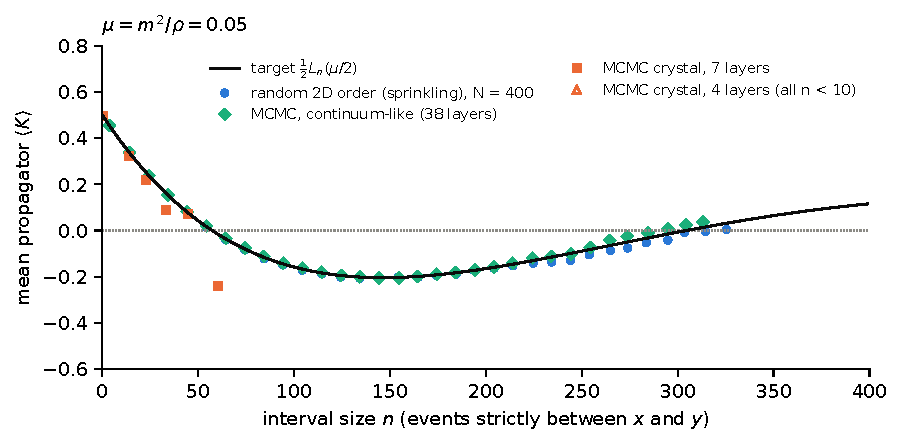
\includegraphics[width=\columnwidth]{fig_laguerre}
\caption{Johnston's propagator averaged over related pairs with interval size $n$, against $\tfrac12L_n(\mu/2)$, at $\mu=0.05$ and $N=400$. At large $n$ few pairs remain and the bins are noisy. In the 4-layer crystal every interval has fewer than 10 elements, so it contributes a single point near $n=0$.}
\label{fig:laguerre}
\end{figure}

\section{Other approaches tested}\label{app:dropped}
\begin{itemize}
\item \emph{Fixed-$n$ propagator as a curvature estimator.} In curved $1+1$ spacetime a term $(R\tau^2/48)J_2(m\tau)$ appears in the propagator~\cite{NXDS17}. In a de Sitter diamond conditioned on $n$ elements the order depends only on $(n,H\tau)$, so a fixed-$n$ curvature test exists. We find that the fraction of related pairs rises by $\approx0.027\,(H\tau)^2$ for $n=10$--$60$, and that the fixed-$n$ propagator is no more sensitive than that fraction alone: a $3\sigma$ detection at $n=30$, $H\tau=1$ requires 175 intervals in either case. The fixed-$n$ propagator therefore detects curvature only through the known chain-abundance route~\cite{RSS13}.
\item \emph{Embedding test on small orders.} We first applied the test to exhaustive ensembles of small orders ($N\leq12$). Its statistics do not separate flat from layered orders at these sizes, and only settle for $N\gtrsim100$ [Fig.~\ref{fig:detector}(a)], so we moved to Monte Carlo samples at $N\geq200$.
\item \emph{Hysteresis in the $e^{-\beta S}$ chains.} At $N=400$, chains started from random and from layered orders at the same $\beta$ end in different phases. We first read this as hysteresis of the transition; the chains from layered starts accept $\leq0.1\%$ of the moves and are effectively frozen, so the difference reflects the sampler rather than the model.
\item \emph{Two-dimensional estimator on $2+1$ sprinklings.} Fed into the embedding, Eq.~\eqref{eq:est} applied to a $2+1$ sprinkling (with the $2+1$ density) produces two large positive eigenvalues. The formula is not valid there, so this is at most a qualitative indication that the spectrum counts spatial dimensions.
\end{itemize}

\begin{thebibliography}{99}
\bibitem{BLMS87} L.~Bombelli, J.~Lee, D.~Meyer, and R.~D.~Sorkin, Space-time as a causal set, Phys.\ Rev.\ Lett.\ \textbf{59}, 521 (1987).
\bibitem{Surya19} S.~Surya, The causal set approach to quantum gravity, Living Rev.\ Relativ.\ \textbf{22}, 5 (2019), arXiv:1903.11544.
\bibitem{BrightwellGregory91} G.~Brightwell and R.~Gregory, Structure of random discrete spacetime, Phys.\ Rev.\ Lett.\ \textbf{66}, 260 (1991).
\bibitem{Myrheim78} J.~Myrheim, Statistical geometry, CERN Report No.\ TH-2538, 1978.
\bibitem{Meyer88} D.~A.~Meyer, The dimension of causal sets, Ph.D.\ thesis, Massachusetts Institute of Technology, 1988.
\bibitem{RSS13} M.~Roy, D.~Sinha, and S.~Surya, Discrete geometry of a small causal diamond, Phys.\ Rev.\ D \textbf{87}, 044046 (2013), arXiv:1212.0631.
\bibitem{GlaserSurya13} L.~Glaser and S.~Surya, Towards a definition of locality in a manifoldlike causal set, Phys.\ Rev.\ D \textbf{88}, 124026 (2013), arXiv:1309.3403.
\bibitem{BD10} D.~M.~T.~Benincasa and F.~Dowker, The scalar curvature of a causal set, Phys.\ Rev.\ Lett.\ \textbf{104}, 181301 (2010), arXiv:1001.2725.
\bibitem{DowkerGlaser13} F.~Dowker and L.~Glaser, Causal set d'Alembertians for various dimensions, Classical Quantum Gravity \textbf{30}, 195016 (2013), arXiv:1305.2588.
\bibitem{BK24} M.~Bogu\~n\'a and D.~Krioukov, Measuring spatial distances in causal sets via causal overlaps, Phys.\ Rev.\ D \textbf{110}, 024008 (2024), arXiv:2401.17376.
\bibitem{RideoutWallden09} D.~Rideout and P.~Wallden, Spacelike distance from discrete causal order, Classical Quantum Gravity \textbf{26}, 155013 (2009), arXiv:0810.1768.
\bibitem{MRS06} S.~Major, D.~Rideout, and S.~Surya, Spatial hypersurfaces in causal set cosmology, Classical Quantum Gravity \textbf{23}, 4743 (2006), arXiv:gr-qc/0506133.
\bibitem{MRS07} S.~Major, D.~Rideout, and S.~Surya, On recovering continuum topology from a causal set, J.\ Math.\ Phys.\ \textbf{48}, 032501 (2007), arXiv:gr-qc/0604124.
\bibitem{ESV19} A.~Eichhorn, S.~Surya, and F.~Versteegen, Induced spatial geometry from causal structure, Classical Quantum Gravity \textbf{36}, 105005 (2019), arXiv:1809.06192.
\bibitem{KhetrapalSurya13} S.~Khetrapal and S.~Surya, Boundary term contribution to the volume of a small causal diamond, Classical Quantum Gravity \textbf{30}, 065005 (2013), arXiv:1212.0629.
\bibitem{GlaserSurya16} L.~Glaser and S.~Surya, The Hartle--Hawking wave function in 2D causal set quantum gravity, Classical Quantum Gravity \textbf{33}, 065003 (2016), arXiv:1410.8775.
\bibitem{Glaser18} L.~Glaser, The Ising model coupled to 2d orders, Classical Quantum Gravity \textbf{35}, 084001 (2018), arXiv:1802.02519.
\bibitem{Glaser23} L.~Glaser, Computer simulations of causal sets, arXiv:2306.09904 (2023).
\bibitem{HMM25} C.~A.~Hu, D.~A.~Meyer, and E.~J.~Q.~Meyer, Reconstructing Minkowski geometry from causal separations, J.\ Math.\ Phys.\ \textbf{66}, 122502 (2025), arXiv:2601.03280.
\bibitem{CloughEvans16} J.~R.~Clough and T.~S.~Evans, Embedding graphs in Lorentzian spacetime, PLoS One \textbf{12}, e0187301 (2017), arXiv:1602.03103.
\bibitem{Clough17} J.~R.~Clough, Causal structure in networks, Ph.D.\ thesis, Imperial College London, 2017, hdl:10044/1/50162.
\bibitem{Henson06} J.~Henson, Constructing an interval of Minkowski space from a causal set, Classical Quantum Gravity \textbf{23}, L29 (2006), arXiv:gr-qc/0601069.
\bibitem{Johnston25} S.~Johnston, Simpler embeddings of causal sets into Minkowski spacetime, Phys.\ Rev.\ D \textbf{111}, 106020 (2025), arXiv:2502.09701.
\bibitem{Johnston08} S.~Johnston, Particle propagators on discrete spacetime, Classical Quantum Gravity \textbf{25}, 202001 (2008), arXiv:0806.3083.
\bibitem{Johnston09} S.~Johnston, Feynman propagator for a free scalar field on a causal set, Phys.\ Rev.\ Lett.\ \textbf{103}, 180401 (2009), arXiv:0909.0944.
\bibitem{BHS08} G.~Brightwell, J.~Henson, and S.~Surya, A 2D model of causal set quantum gravity: the emergence of the continuum, Classical Quantum Gravity \textbf{25}, 105025 (2008), arXiv:0706.0375.
\bibitem{Surya12} S.~Surya, Evidence for the continuum in 2D causal set quantum gravity, Classical Quantum Gravity \textbf{29}, 132001 (2012), arXiv:1110.6244.
\bibitem{GOS18} L.~Glaser, D.~O'Connor, and S.~Surya, Finite size scaling in 2d causal set quantum gravity, Classical Quantum Gravity \textbf{35}, 045006 (2018), arXiv:1706.06432.
\bibitem{Embedding} R.~Bada, Spatial embedding of $3+1$ causal sets: low-count spacelike pairs and a likelihood fit to interval counts (companion paper, 2026), to be submitted.
\bibitem{BDJ99} J.~Baik, P.~Deift, and K.~Johansson, On the distribution of the length of the longest increasing subsequence of random permutations, J.\ Am.\ Math.\ Soc.\ \textbf{12}, 1119 (1999).
\bibitem{Cunningham18} W.~J.~Cunningham, Inference of boundaries in causal sets, Classical Quantum Gravity \textbf{35}, 094002 (2018), arXiv:1710.09705.
\bibitem{BBR26} J.~Barton, S.~Borza, and J.~R\"ohrig, Ollivier--Ricci curvature for causal sets, arXiv:2606.04910 (2026).
\DIFaddbegin \bibitem{LastPenrose17} \DIFadd{G.~Last and M.~Penrose, }\emph{\DIFadd{Lectures on the Poisson Process}} \DIFadd{(Cambridge University Press, Cambridge, 2017), Ch.~4.
}\DIFaddend \bibitem{Pinsky06} R.~G.~Pinsky, Law of large numbers for increasing subsequences of random permutations, Random Struct.\ Algorithms \textbf{29}, 277 (2006), arXiv:math/0407353, Eq.~(1.1).
\bibitem{Szego39} G.~Szeg\H{o}, \emph{Orthogonal Polynomials}, American Mathematical Society Colloquium Publications Vol.~23 (AMS, New York, 1939).
\bibitem{LifschitzPittel81} V.~Lifschitz and B.~Pittel, The number of increasing subsequences of the random permutation, J.\ Comb.\ Theory Ser.\ A \textbf{31}, 1 (1981).
\bibitem{OEIS} OEIS Foundation, The On-Line Encyclopedia of Integer Sequences, sequence A002720, \url{https://oeis.org/A002720}.
\bibitem{ABP18} M.~E.~Aghili, L.~Bombelli, and B.~B.~Pilgrim, Path length distribution in two-dimensional causal sets, Eur.\ Phys.\ J.\ C \textbf{78}, 744 (2018), arXiv:1805.07312.
\bibitem{Shuman23} S.~Shuman, Path sums for propagators in causal sets, Phys.\ Rev.\ D \textbf{109}, 046008 (2024), arXiv:2307.08864.
\bibitem{KastratiHinrichsen26} A.~Kastrati and H.~Hinrichsen, Numerical evaluation of the causal set propagator in 2D anti-de Sitter spacetime, Phys.\ Rev.\ D \textbf{113}, 065003 (2026), arXiv:2504.12919.
\bibitem{EMLW26} A.~Eichhorn, H.~Mack, K.~T.~Le, and F.~Wagner, Charting causal set configuration space with graph observables, arXiv:2605.27514 (2026).
\bibitem{RideoutSorkin00} D.~P.~Rideout and R.~D.~Sorkin, Classical sequential growth dynamics for causal sets, Phys.\ Rev.\ D \textbf{61}, 024002 (2000).
\bibitem{MORS01} X.~Mart\'in, D.~O'Connor, D.~P.~Rideout, and R.~D.~Sorkin, On the renormalization transformations induced by cycles of expansion and contraction in causal set cosmology, Phys.\ Rev.\ D \textbf{63}, 084026 (2001).
\bibitem{AhmedRideout10} M.~Ahmed and D.~Rideout, Indications of de Sitter spacetime from classical sequential growth dynamics of causal sets, Phys.\ Rev.\ D \textbf{81}, 083528 (2010).
\bibitem{CunninghamSurya19} W.~J.~Cunningham and S.~Surya, Dimensionally restricted causal set quantum gravity: examples in two and three dimensions, Classical Quantum Gravity \textbf{37}, 054002 (2020), arXiv:1908.11647.
\bibitem{NXDS17} Nomaan~X, F.~Dowker, and S.~Surya, Scalar field Green functions on causal sets, Classical Quantum Gravity \textbf{34}, 124002 (2017), arXiv:1701.07212.
\bibitem{MethodNote} R.~Bada, Two causal-set papers written with an AI research partner: methodology note (2026), \DIFdelbegin \DIFdel{to be }\DIFdelend released with the code at \url{https://github.com/presindev/causet-counting}.
\end{thebibliography}

\end{document}
